\section{~Input data}

Exclusive bare hadronic cross-section measurements for 32 channels are integrated up to 1.8$\;$GeV over the relevant dispersion kernels. This analysis uses all the available public data with recent additions~\cite{CMD-3:2017tgb,TheBaBar:2017vzo,Achasov:2017vaq,cleo2017,TheBABAR:2018vvb,Achasov:2018ujw,Lees:2018dnv,cmd3-7pi,Achasov:2019duv,Ivanov:2019crp}. References for data already included in our 2017 analysis are provided in the corresponding paper~\cite{dhmz2017} as well as earlier publications~\cite{dhmz2011,dehz2003}.

In the energy range 1.8--3.7$\;$GeV and above 5$\;$GeV four-loop perturbative QCD is used~\cite{baikov}. The contributions from the open charm pair production region between 3.7 and 5$\;$GeV are again computed using experimental data. For the narrow resonances $J/\psi$ and $\psi(2S)$ Breit-Wigner line shapes are integrated using their currently best known parameters~\cite{pdg}.

The following  discussion of individual channels  focuses on the HVP contribution to $\amu$ as it relies more strongly on the low-energy experimental data. We mainly explore the impact of the  data released since our last publications~\cite{dhmz2017,dhmz2011}. If not stated otherwise, all numerical results for \amu are quoted in units of $10^{-10}$.

\begin{figure*}[p]
\begin{center}
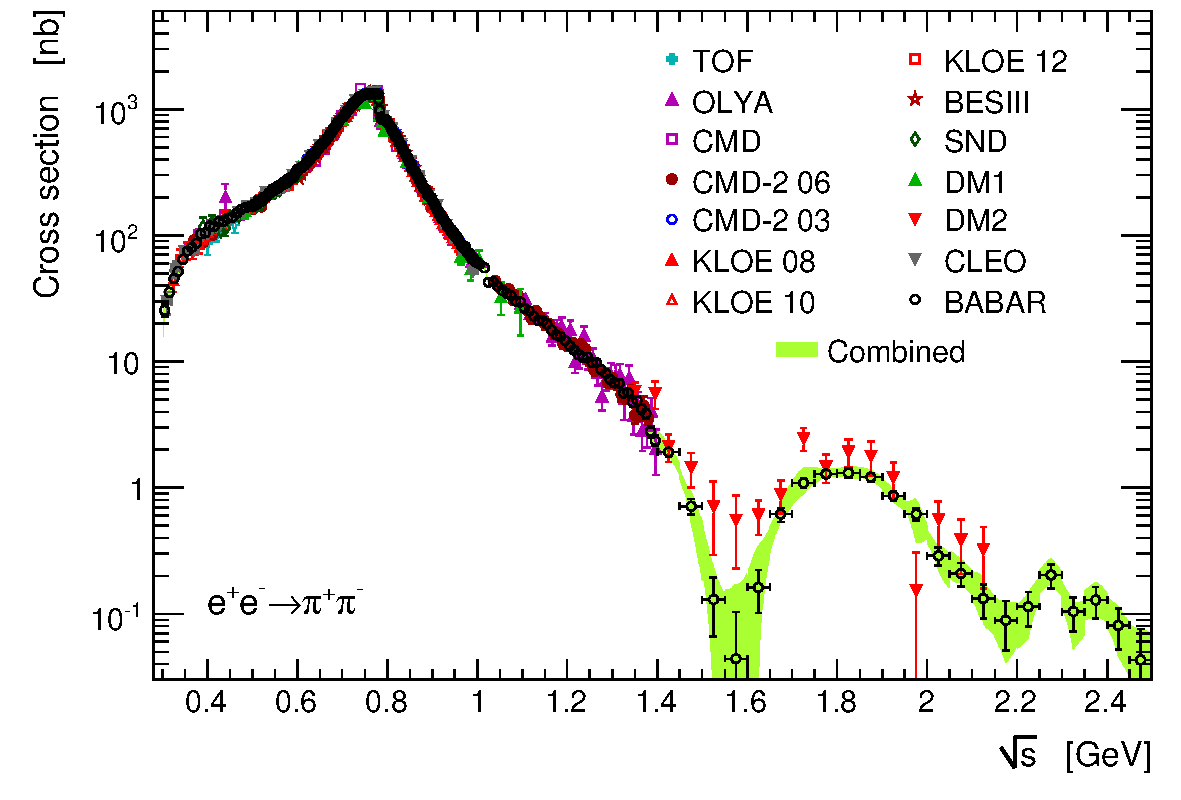
\includegraphics[width=130mm]{Figures/combined_2pi_ePeM_to_piPpiM_log0,28-2,5GeV_dhmz19.pdf}
\vspace{0.5cm}

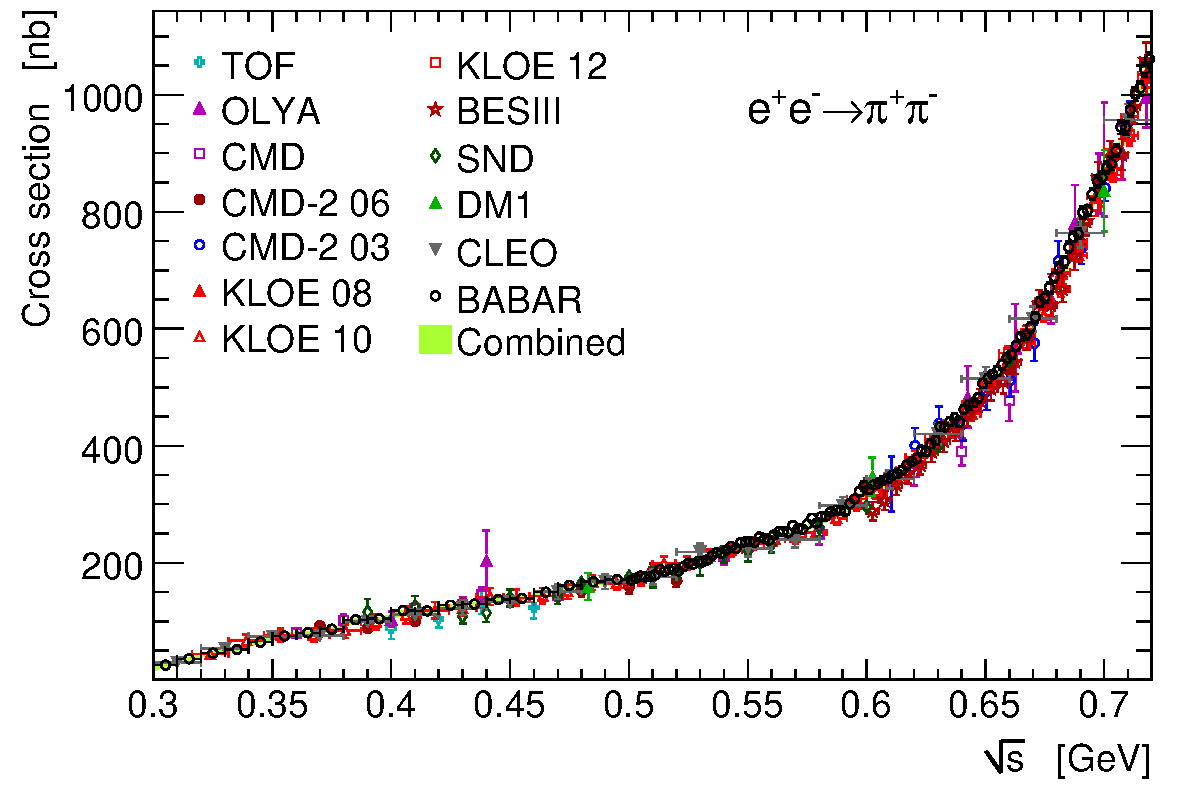
\includegraphics[width=\figsize]{Figures/combined_2pi_ePeM_to_piPpiM_0,3-0,72GeV_dhmz19.pdf}\hspace{\fighspace}
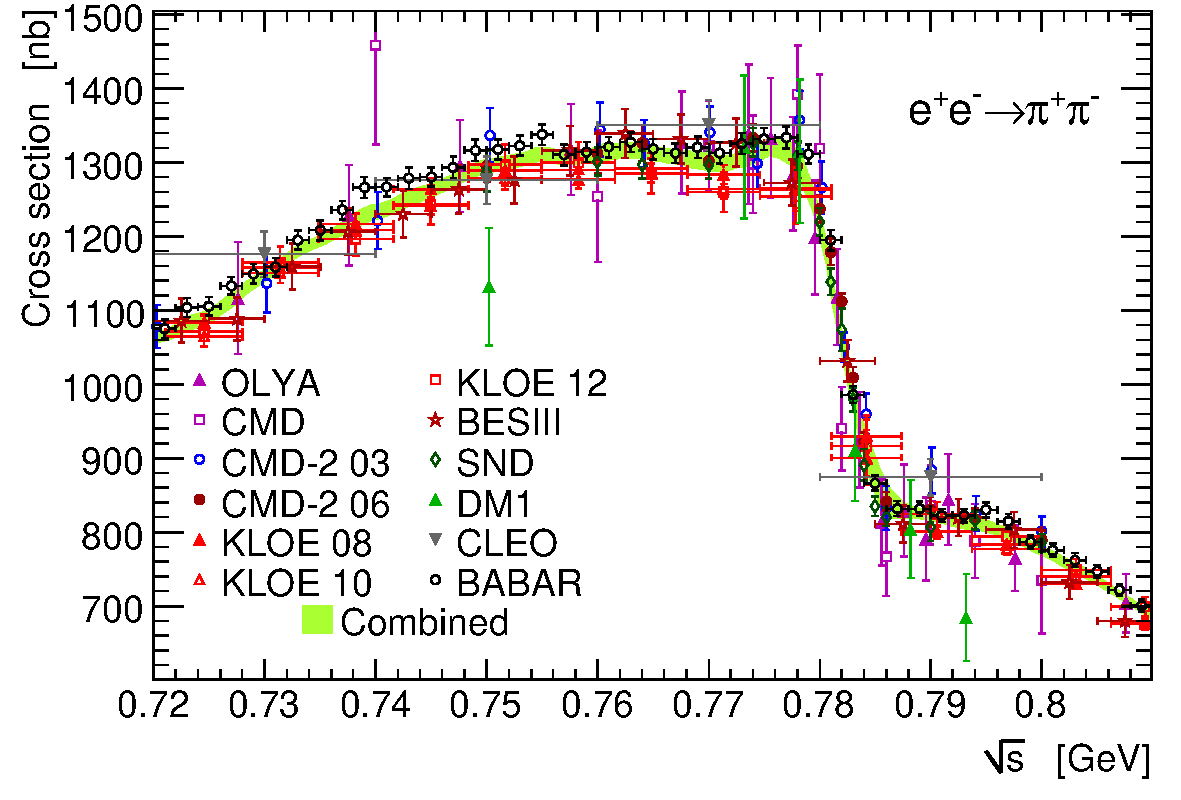
\includegraphics[width=\figsize]{Figures/combined_2pi_ePeM_to_piPpiM_0,72-0,81GeV_dhmz19.pdf}
\vspace{0.2cm}

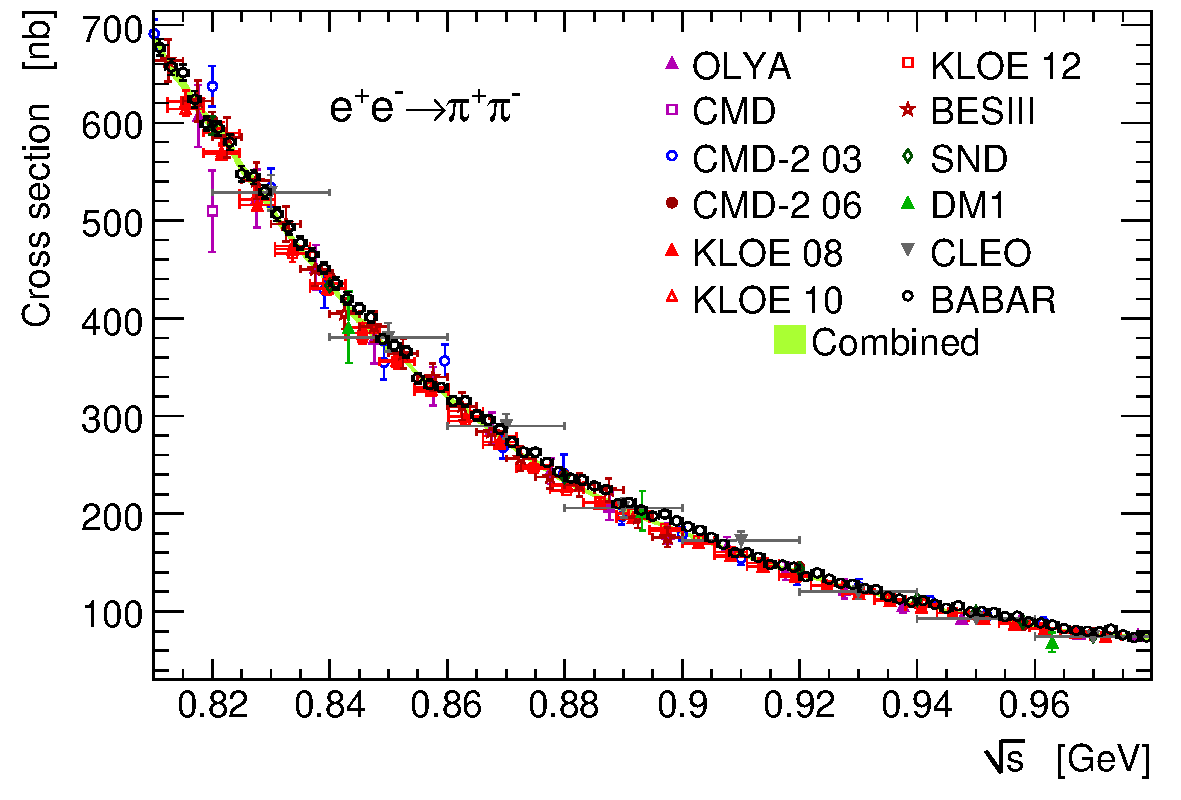
\includegraphics[width=\figsize]{Figures/combined_2pi_ePeM_to_piPpiM_0,81-0,98GeV_dhmz19.pdf}\hspace{\fighspace}
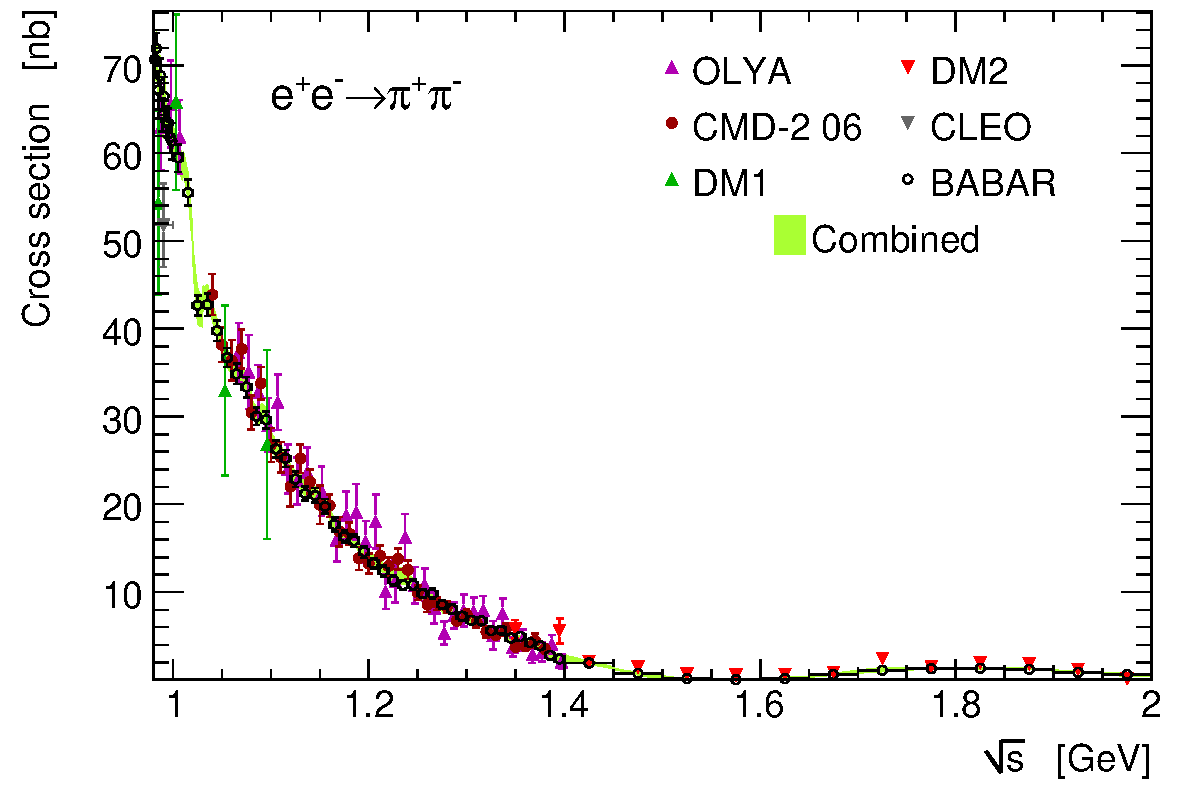
\includegraphics[width=\figsize]{Figures/combined_2pi_ePeM_to_piPpiM_0,98-2,0GeV_dhmz19.pdf}
\end{center}
\vspace{-0.2cm}
\caption[.]{ 
            Bare cross section of $\ee\to\pp$ versus centre-of-mass energy for different 
            energy ranges.  The error bars of the data points include statistical and systematic 
            uncertainties added in quadrature. The green band shows
            the HVPTools combination within its $1\sigma$ uncertainty. 
    
}
\label{fig:pipiall}
\end{figure*}
\begin{figure*}[p]
\begin{center}
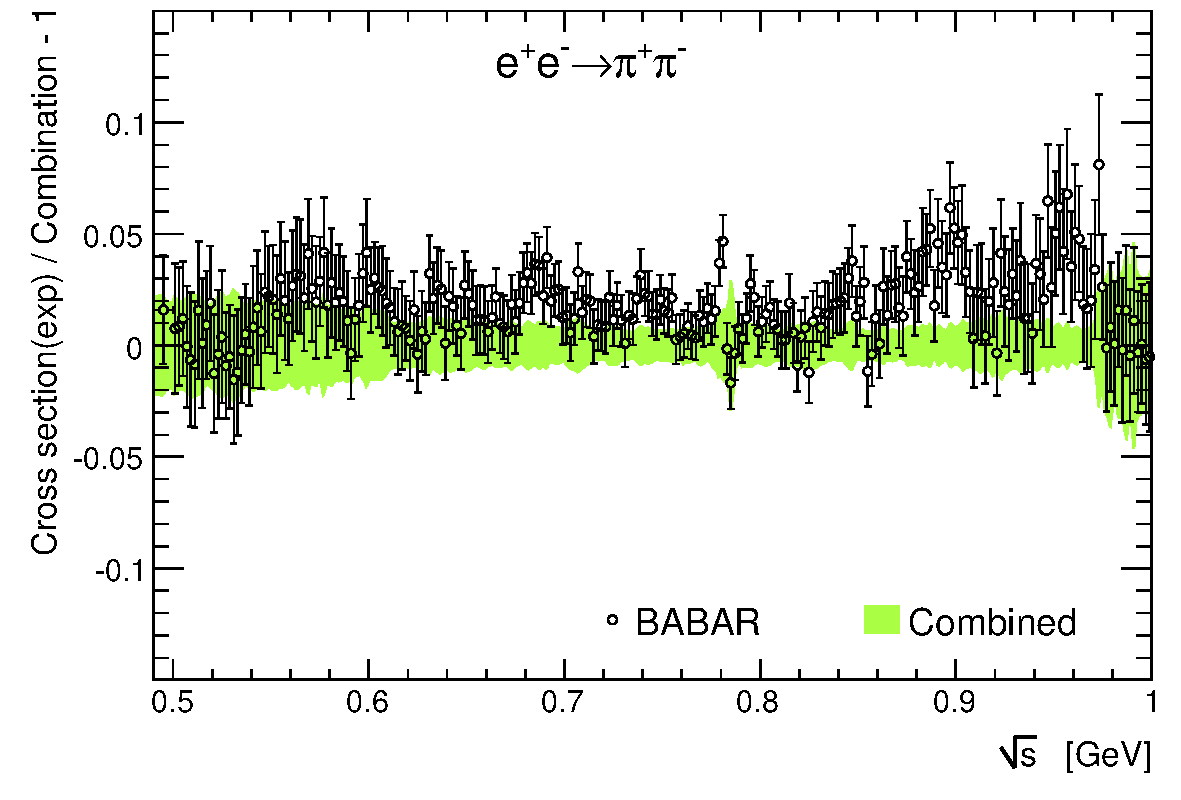
\includegraphics[width=\figsize]{Figures/diffRel_channel_ePeM_to_piPpiM_babar_dhmz19.pdf}\hspace{\fighspace}
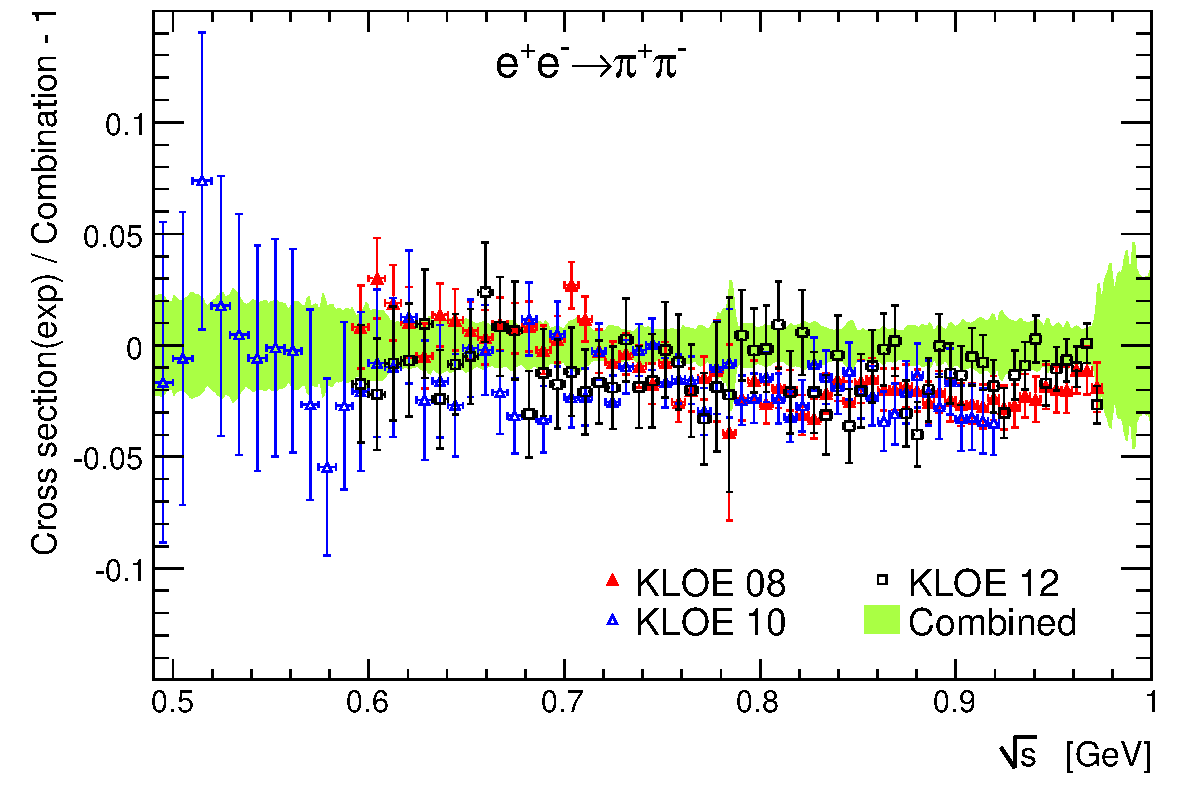
\includegraphics[width=\figsize]{Figures/diffRel_channel_ePeM_to_piPpiM_kloe_dhmz19.pdf}
\vspace{0.2cm}

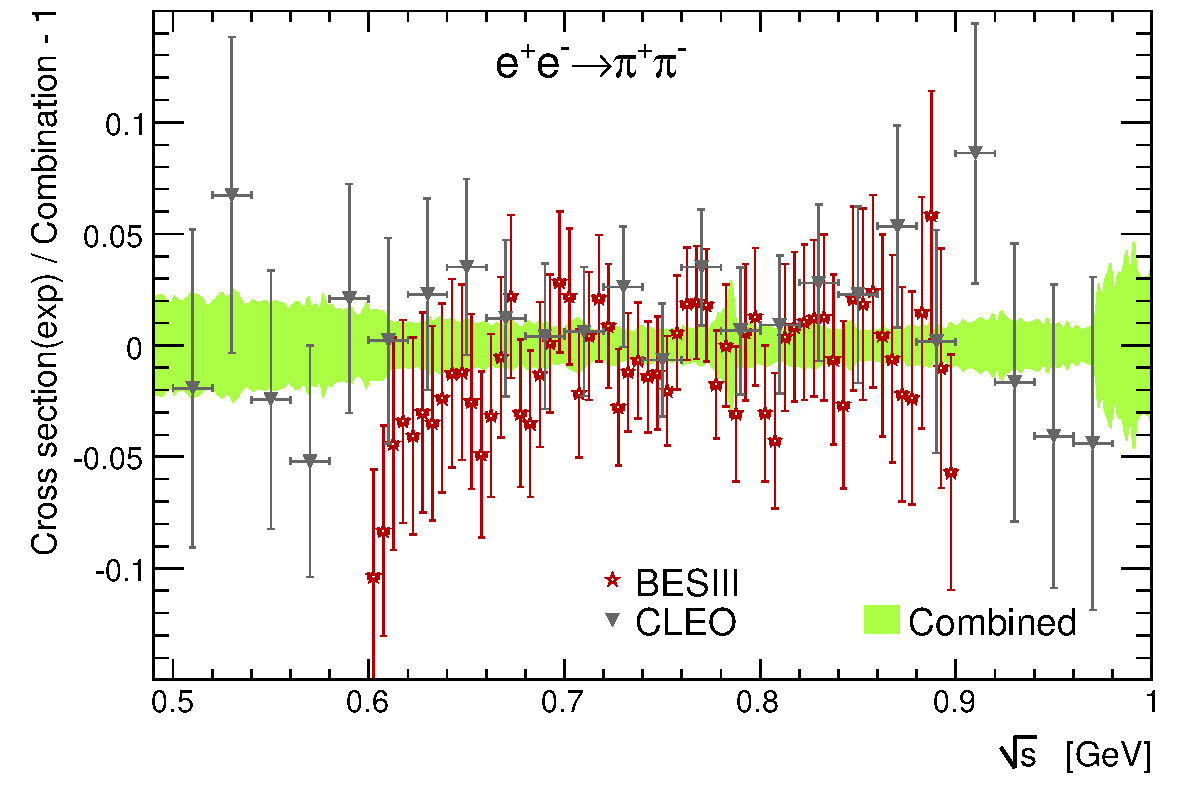
\includegraphics[width=\figsize]{Figures/diffRel_channel_ePeM_to_piPpiM_bescleo_dhmz19.pdf}\hspace{\fighspace}
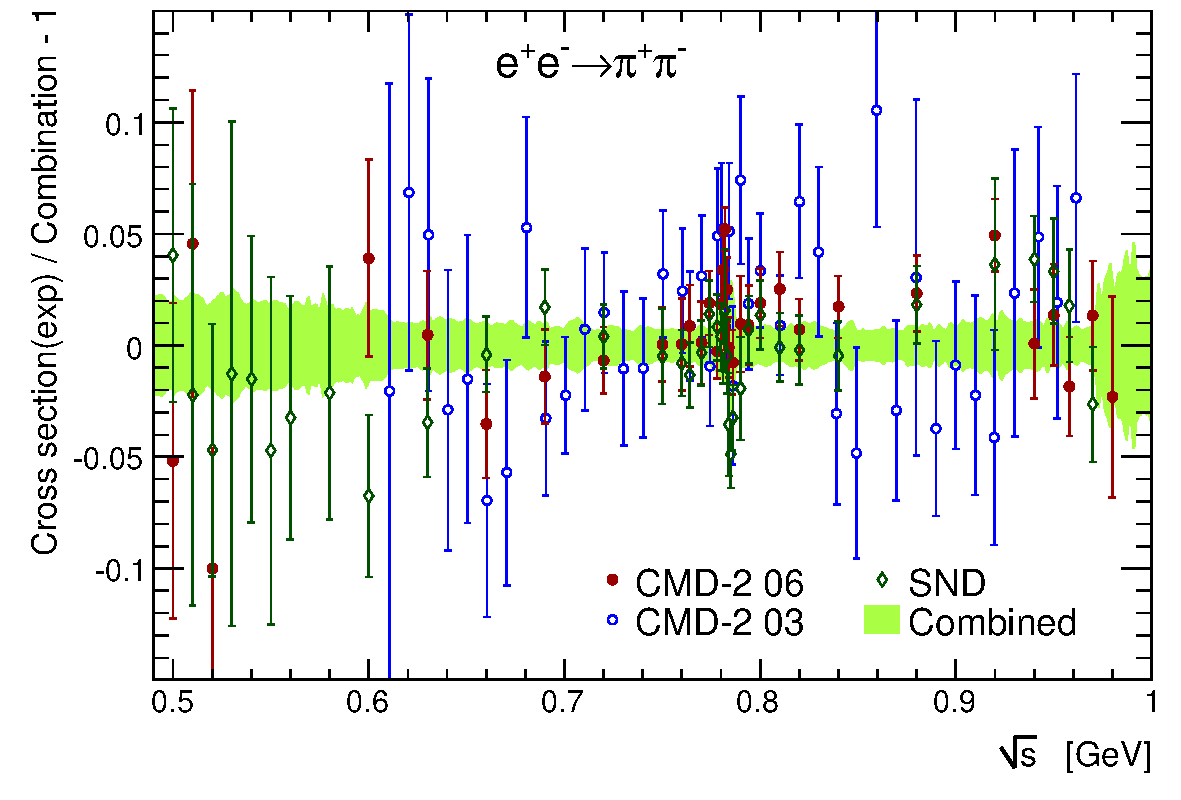
\includegraphics[width=\figsize]{Figures/diffRel_channel_ePeM_to_piPpiM_CMD2SND_dhmz19.pdf}
\end{center}
\vspace{-0.2cm}
\caption[.]{ 
            Comparison between individual $\ee\to\pp$ cross-section measurements from 
            BABAR~\cite{babarpipi1,babarpipi2},  KLOE\,08~\cite{kloe08}, KLOE\,10~\cite{kloe10},
            KLOE\,12~\cite{kloe12}, BESIII~\cite{bes2015}, CLEO~\cite{cleo2017},
            CMD-2\,03~\cite{cmd203}, CMD-2\,06~\cite{cmd2new}, SND~\cite{snd2pi}, and 
            the HVPTools combination. The error bars include statistical and systematic 
            uncertainties added in quadrature. 
}
\label{fig:comppipi}
%\end{figure*}
%\begin{figure*}[t]
\vspace{1.5cm}
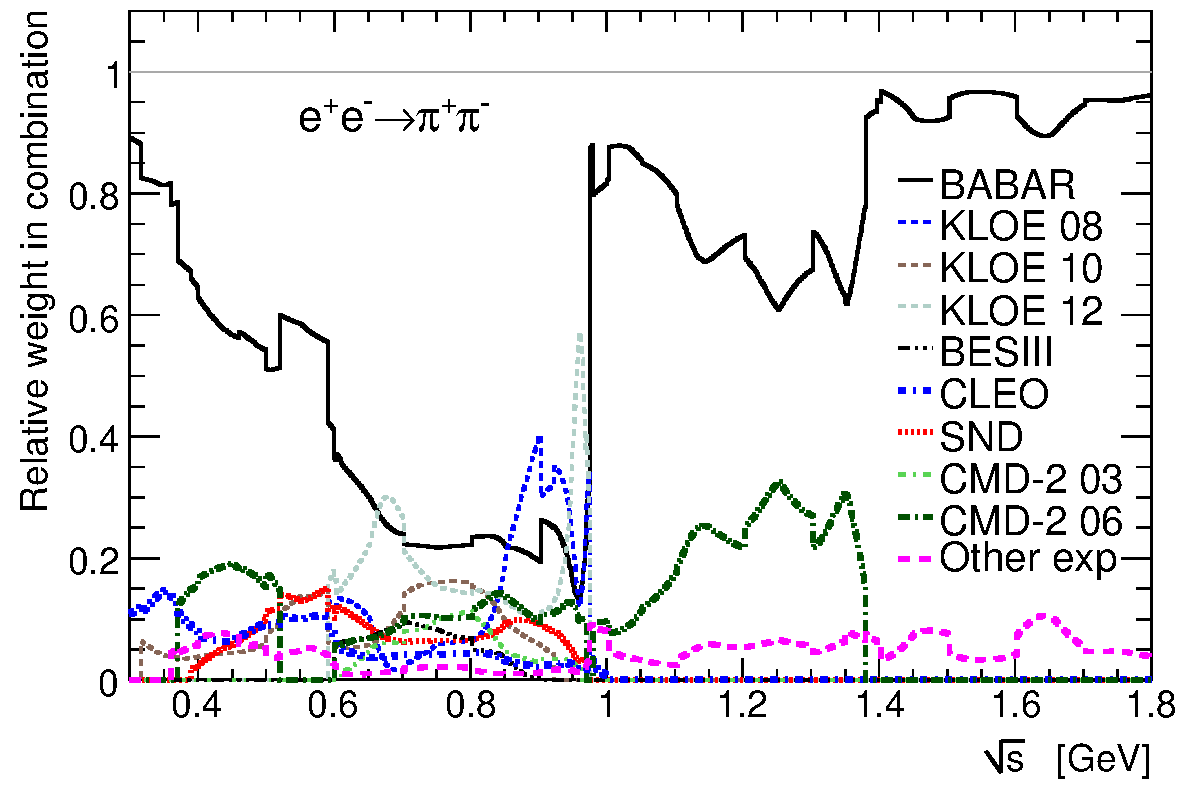
\includegraphics[width=\figsize]{Figures/Weights_2pi_dhmz19.pdf}\hspace{\fighspace}
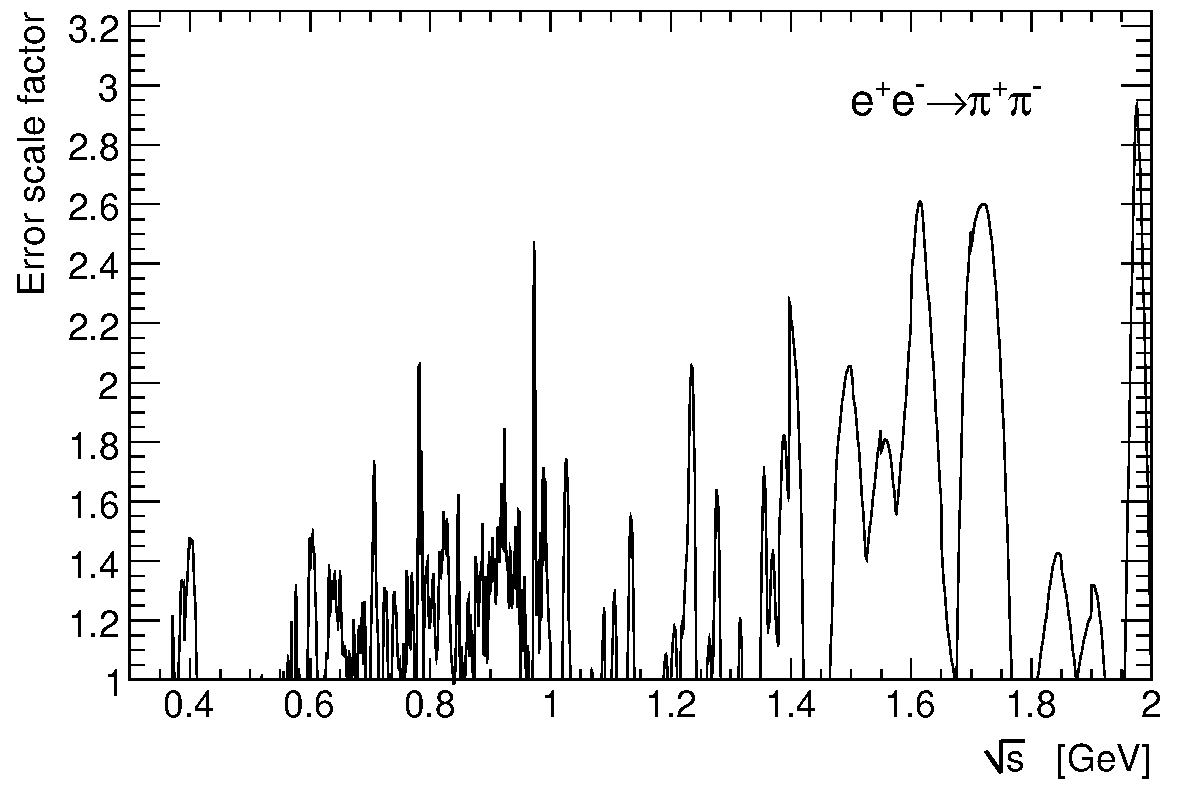
\includegraphics[width=\figsize]{Figures/Chi2Correction_combined_ePeM_to_piPpiM_dhmz19.pdf}
\vspace{0.1cm}

\caption[.]{ 
            Left: relative local weight per experiment contributing to the $\ee\to\pp$
            cross-section combination versus centre-of-mass energy. 
            Right: local scale factor versus centre-of-mass energy applied 
            to the combined \pp cross-section uncertainty to account for inconsistency 
            in the individual measurements. }
\label{fig:weights}
\end{figure*}


\subsection{~The \sansmath$\mathbf{\boldsymbol{\pi^+\pi^-}}$ channel}
\label{sec:pipi}

Data from the BABAR~\cite{babarpipi1,babarpipi2} and KLOE~\cite{kloe08,kloe10,kloe12} experiments dominate  the measurement of the \pp channel. Their  sub-percent precision is not matched by the other experiments (CMD-2, SND, and BESIII\footnote{There is a small inconsistency between the bin-by-bin statistical uncertainties and the diagonal values of the statistical covariance matrix of the \pp data published by BESIII~\cite{bes2015}.}). New data in this channel stem from CLEO~\cite{cleo2017} using large angle initial state radiation (ISR) and taking into account up to one additional photon, following the BABAR method~\cite{babarpipi1}. Relatively large statistical uncertainties and a systematic uncertainty of 1.5\% are, however, insufficient to improve the precision of the combined $\pipi$ contribution. Recently, a combination of the three KLOE measurements was proposed~\cite{kloe17}. We do not use this combination as the KLOE measurements correspond to different ISR topologies and normalisation procedures.\footnote{Using the  KLOE combination~\cite{kloe17} we find for \amuhadLOpp  between the \pp threshold and $1.8\;$GeV a value of $506.6 \pm 2.4$, which is to be compared with $506.7 \pm 2.3$ as obtained from the HVPTools combination. For both calculations the usual local $\sqrt{\chiSdof}$ uncertainty rescaling method was applied. Without the rescaling the corresponding results are $506.6 \pm 2.0$ and $506.7 \pm 2.0$, respectively. The similarity of the results is maintained when using a phenomenological fit up to 0.6$\;$GeV (see later in text).} Eigenvector decomposition of the statistical and systematic covariance matrices of the three most recent series of KLOE measurements~\cite{kloe17} is used. Each eigenvector multiplied by the square-root of the corresponding eigenvalue is treated as an uncertainty source that is fully correlated between the  KLOE data points, while the individual sources are treated as independent among each other. Pseudo-experiments are generated in the usual way to propagate correlated uncertainties among the KLOE measurements.

Figure~\ref{fig:pipiall} shows the available $\ee\to\pp$ cross-section measurements in various panels zooming into different energy ranges. The green band indicates the HVPTools combination within its $1\sigma$ uncertainty. Comparisons between the combination and the most precise individual measurements are plotted in Fig.~\ref{fig:comppipi}. Figure~\ref{fig:weights} (left) shows the local combination weight versus $\sqrt{s}$ per experiment. The BABAR and KLOE measurements dominate over the entire energy range. Owing to the sharp radiator function, the KLOE event yield  increases towards the $\phi(1020)$ mass leading to a better precision than BABAR in the 0.8$-$1.0 GeV region. The group of experiments labelled ``Other exp'' in the left panel of Fig.~\ref{fig:weights} corresponds to older data with incomplete radiative corrections. Their weights are small throughout the entire energy domain. The right hand panel of Fig.~\ref{fig:weights} shows the scale factor versus centre-of-mass energy that is locally applied to the combined  \pp cross-section uncertainty to account for inconsistencies among the individual measurements. Significant inconsistencies are found between the most precise BABAR and KLOE datasets. 

The computation of the dispersion integral over the full \pp spectrum requires to extend the available data to the region between threshold and $0.3\:\gev$, for which we use a fit as described below.


\subsubsection*{Phenomenological fit}

\begin{figure*}[t]
\begin{center}
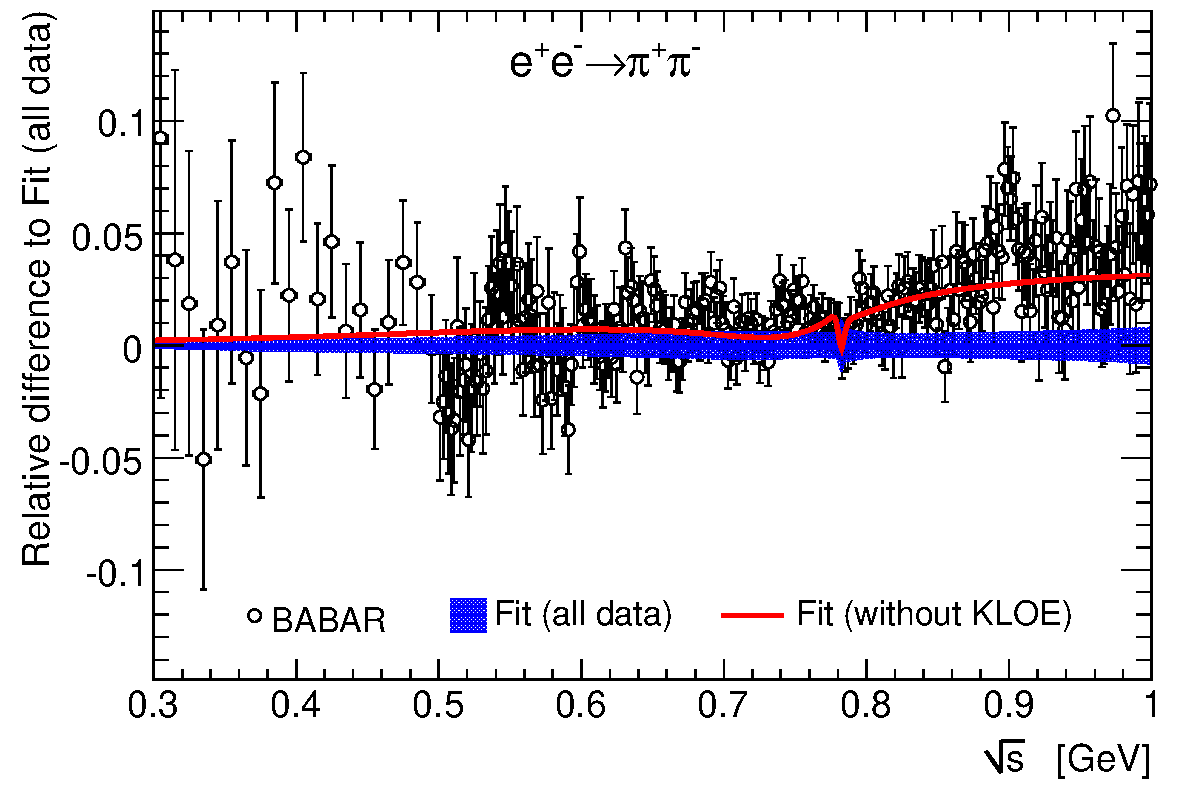
\includegraphics[width=\figsize]{Figures/ff2_fit_babar_dhmz19.pdf}\hspace{\fighspace}
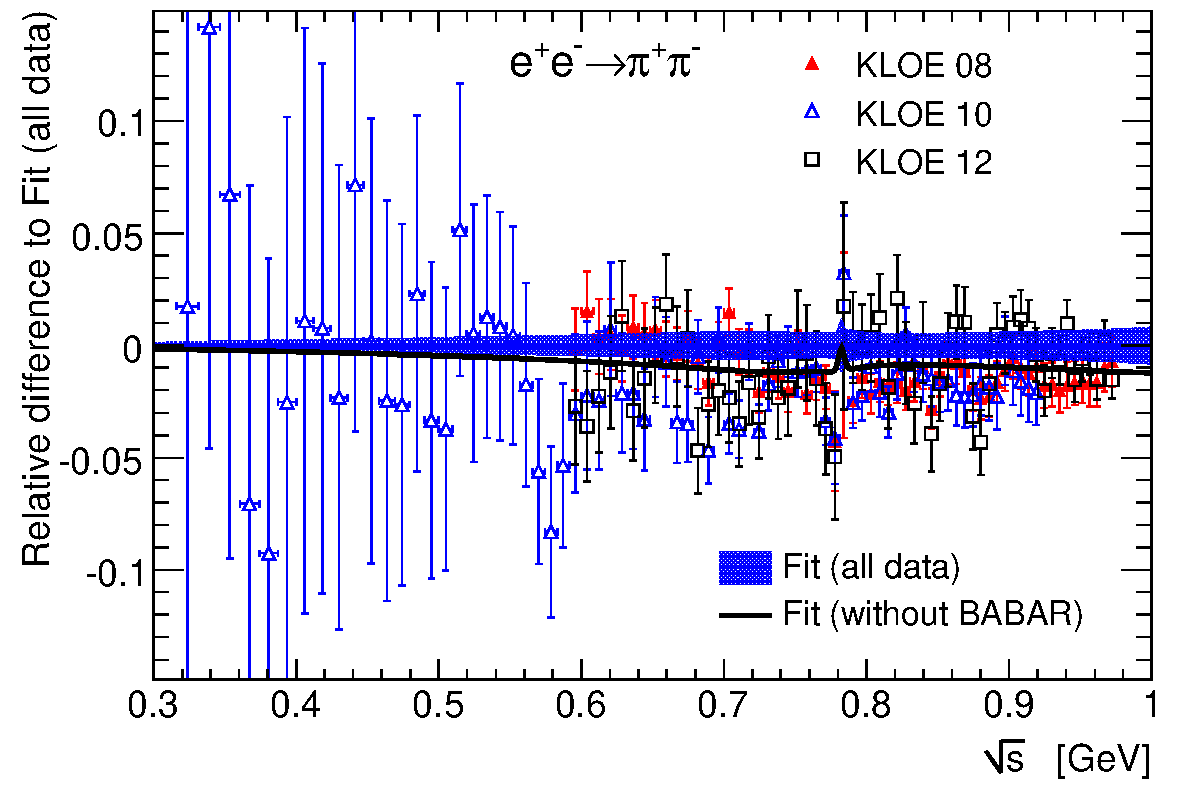
\includegraphics[width=\figsize]{Figures/ff2_fit_kloe_dhmz19.pdf}
\vspace{0.2cm}

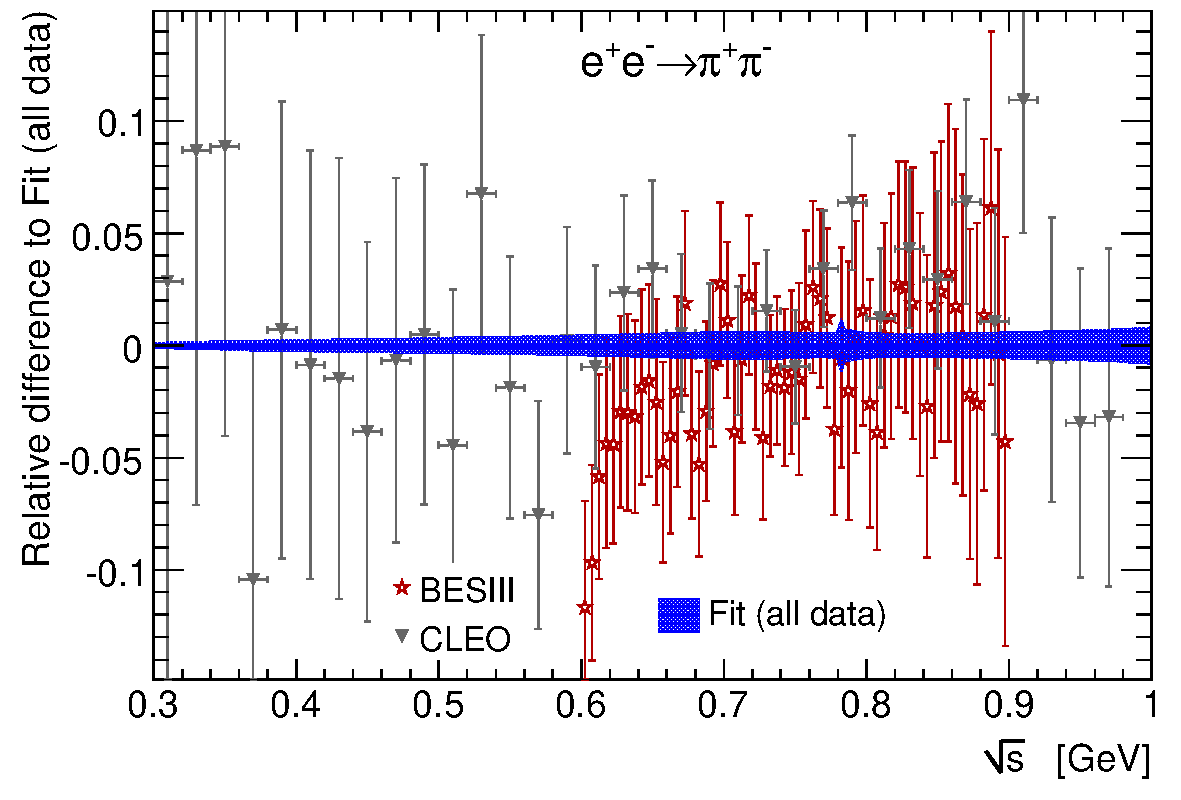
\includegraphics[width=\figsize]{Figures/ff2_fit_bescleo_dhmz19.pdf}\hspace{\fighspace}
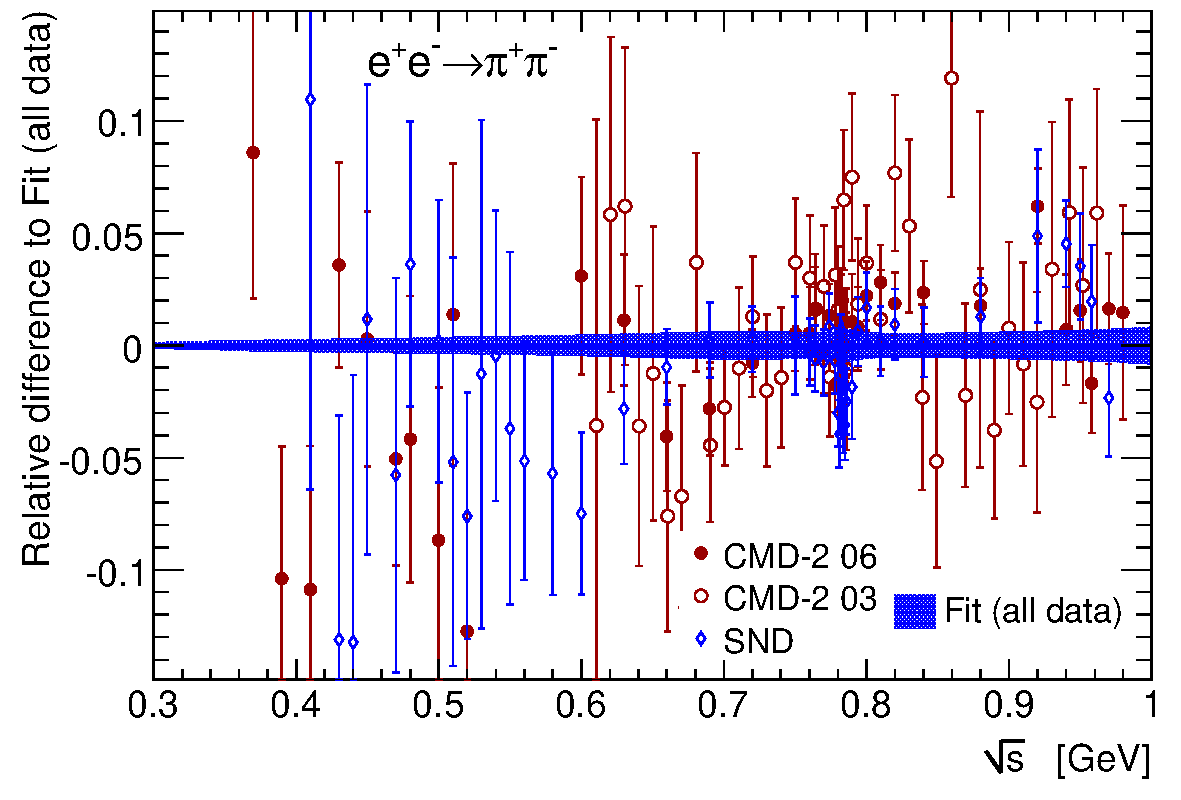
\includegraphics[width=\figsize]{Figures/ff2_fit_sndcmd2_dhmz19.pdf}
\end{center}
\vspace{-0.2cm}
\caption[.]{ 
            Same as Fig.~\ref{fig:comppipi} except that the comparison is made with respect to the fit instead of the combination.
            The black and red curves show the results of two alternative fits where the data from KLOE and BABAR, respectively, were excluded.
}
\label{fig:data-fit}
\end{figure*}
The bare $e^+e^-\to\pp$ annihilation cross section is related to the pion form factor $F^0_\pi(s)$ (excluding vacuum polarisation) by
\begin{eqnarray}
    &&\sigma^{(0)}(e^+e^-\to \pi^+\pi^-)= \nonumber\\
      &&\hspace{1.5cm}\frac{\pi\alpha^2}{3s}\beta^3_0(s)\cdot|F^0_\pi(s)|^2\cdot\textrm{FSR}(s)\,,
\end{eqnarray}
where $\alpha$ is the electromagnetic coupling constant,  $\beta_0(s)=\sqrt{1-4m_\pi^2/s}$ is a threshold kinematic factor and FSR$(s)$ is the final state radiation contribution.

The pion form factor is an analytic function of $s$ in the complex plane, except on the real axis above $4m^2_\pi$. It can be parameterised as a product of two functions~\cite{Hanhart:2016pcd}
\begin{equation}
    F^0_\pi=G(s)\cdot J(s)\,,
    \label{Eq:FeRJ}
\end{equation}
where
\begin{eqnarray}
G(s)&=&1+\alpha_V s + \frac{\kappa s}{m^2_\omega -s -im_\omega\Gamma_\omega}\label{eq:rs}\,,
\end{eqnarray}
and, exploiting the unitarity constraint which identifies ${\rm arg}(F_\pi^0)$ with the P-wave \pp phase shift $\delta_1(s)$, 
\begin{eqnarray}
J(s)&=&e^{1-\delta_1(s_0)/\pi}\cdot\left(1-\frac{s}{s_0}\right)^{\!\!\left[1-\frac{\delta_1(s_0)}{\pi}\right]\frac{s_0}{s}}\!\!\left(1-\frac{s}{s_0}\right)^{\!\!-1}\nonumber\\
&& \cdot\; {\rm exp}\left({\frac{s}{\pi}\int^{s_0}_{4m^2_\pi}dt\frac{\delta_1(t)}{t(t-s)}}\right).\label{eq:js}
\end{eqnarray}
The last term in Eq.~(\ref{eq:rs}) accounts for $\rho-\omega$ mixing. The function $J(s)$ is taken from Refs.~\cite{DeTroconiz:2001rip,deTroconiz:2004yzs}. Owing to $\rho$ dominance, the phase shift $\delta_1(s)$ can be parameterised by~\cite{GarciaMartin:2011cn}
\begin{equation}
    \cot\delta_1(s)=\frac{\sqrt{s}}{2k^3(s)}\left(m^2_\rho-s\right)\left(\frac{2m^3_\pi}{m^2_\rho\sqrt{s}}+B_0+B_1\omega(s)\right)\label{eq:phase}
\end{equation}
with
\begin{eqnarray}
&& k(s)=\frac{\sqrt{s-4m^2_\pi}}{2}\nonumber\,,~~~ \omega(s)=\frac{\sqrt{s}-\sqrt{s_0-s}}{\sqrt{s}+\sqrt{s_0-s}}\,.
\end{eqnarray}
The six free parameters $\alpha_V$, $\kappa$, $m_\omega$, $m_\rho$, $B_0$ and $B_1$ are determined by the fit to the \pp data restricted to the region up to 1$\;$GeV to stay below the threshold of significant inelastic channels. The width of the $\omega$ resonance is fixed to its PDG value of 8.49$\;$MeV~\cite{pdg}, and $\sqrt{s_0}=1.05\:$GeV. The results of the fit are given in Table~\ref{tab:fit}. To derive an estimate for the model uncertainty, we independently vary $\sqrt{s_0}$ to 1.3$\;$GeV and remove the linear term $B_1\omega(s)$ from Eq.~(\ref{eq:phase}) since the resulting value of $B_1$ from the nominal fit is consistent with zero. 

The fit is performed using as test statistic a diagonal \chiS function that accounts for the statistical and systematic uncertainties of the experimental measurements.\footnote{For the fit we use the original data provided by each experiment instead of the HVPTools combination.} The same uncertainty rescaling in case of local discrepancies among datasets as for the HVPTools based combination is applied. Correlations are ignored in the test statistic, but accounted for in the uncertainty propagation through a series of pseudo-experiments for each of which the full fit procedure is repeated. This is a conservative procedure, as exploiting correlations in the test statistic would improve the precision of the fit.
Currently, the most precise measurements are dominated by systematic uncertainties, whose size and mass dependence as well as correlation among each other and among data points rely on estimates with somewhat limited precision, as discussed in section~\ref{Sec:Combination}.
Since there are also clear indications of a significant underestimate of the size of uncertainties in the discrepant dataset(s), we prefer not to exploit this information in the constrained fit.
Pseudo-experiments are also used to assess the goodness-of-fit on the data, which yields a p-value of 0.27.\footnote{The p-values for each individual dataset read 0.042 (BABAR), 0.097 (KLOE), 0.449 (CMD), 0.675 (TOF), 0.718 (DM1), 0.756 (CMD-2), 0.796 (SND), and 0.984 (CLEO). The p-values for both OLYA and BESIII are close to 1.}
We have checked the reliability of this procedure by generating a set of pseudo-experiments and evaluating the p-value for each of them.
The expected distribution of p-values reconstructed this way is indeed uniform between $0$ and $1$.

A graphical comparison of the fit result with the data is shown in Fig.~\ref{fig:data-fit}.
\begin{table*}[tbh]
\setlength{\tabcolsep}{0.0pc}
\begin{tabularx}{\textwidth}{@{\extracolsep{\fill}}lrrrrrr} 
\hline\noalign{\smallskip}
 & $\alpha_V$ & $\kappa [10^{-4}]$ & $B_0$ & $B_1$ & $m_\rho$ [MeV] & $m_\omega$ [MeV] \\
\noalign{\smallskip}\hline\noalign{\smallskip}
$\alpha_V$ & $0.133\pm 0.020$ & 0.52 & $-0.45$ & $-0.97$ & 0.90 & $-0.25$ \\
$\kappa [10^{-4}]$ & & $21.6\pm 0.5$ & $-0.33$ & $-0.57$ & 0.64 & $-0.08$ \\
$B_0$ & & & $1.040\pm 0.003$ & 0.40 & $-0.40$ & 0.29 \\
$B_1$ & & & & $-0.13\pm 0.11$ & $-0.96$ & 0.20 \\
$m_\rho$ [MeV] & & & & & $774.5\pm 0.8$ & $-0.17$ \\
$m_\omega$ [MeV] & & & & & & $782.0\pm 0.1$ \\
\noalign{\smallskip}\hline
\end{tabularx}
    \caption{Results of the fit to all $\pi^+\pi^-$ data. The diagonal elements give the fitted parameter values and their uncertainties, while the off-diagonal elements give the correlation coefficients.}
    \label{tab:fit}
\end{table*}
In the energy range between 0.3 and 0.6 GeV, the result of the fit yields for \amuhadLOpp a contribution of $109.8 \pm 0.4\pm 0.4$, where the first error is experimental and the second the model uncertainty. The latter is obtained by adding linearly the absolute values of following two variations: the $\sqrt{s_0}$ variation of $-0.13\pm 0.10$ and the difference of without and with the $B_1\omega(s)$ term of $0.24\pm 0.14$, where the uncertainty of each variation accounts for the correlation between the integral results. The corresponding result based on data integration is $109.6 \pm 1.0$. Taking into account the correlation of $72\%$ between the  experimental uncertainties, the difference between the two evaluations amounts to $0.2 \pm 0.9$. Similarly, for \dahadZ the difference is $0.020 \pm 0.028$. The fit therefore gives compatible but more precise results than the direct data integration.

Other studies using constraints from unitarity and analyticity with the aim to improve the precision of the \pp HVP contribution to the muon $g-2$ exist in the literature.\footnote{In Ref.~\cite{Hoferichter:2019gzf} an analyticity-based phenomenological fit has been used for the $\pi^+\pi^-\pi^0$ channel.}
The treatment followed in Ref.~\cite{Colangelo:2018mtw} is similar to ours with, however, a more elaborate theoretical analysis.
Differences are also present in the treatment of experimental data, Ref.~\cite{Colangelo:2018mtw} using a \chiS computed globally, including correlations across all the experimental data points and bins in the full mass range of interest. However, in order to avoid too low p-values, some bins of the KLOE measurements were removed in that study and energy rescaling parameters were introduced to fit each measured energy spectrum.
A different approach is followed in Ref.~\cite{Ananthanarayan:2018nyx,Ananthanarayan:2019zic} where the low-mass contribution was obtained from input data at a fixed mass, followed by a simple average used to combine inputs in the \sqrtS range between $0.65$ and $0.71$~GeV (and then to combine values from different experiments).
Instead of a direct evaluation of the correlations from the published information, they were assumed to be the same between all the combination inputs and an attempt was made to evaluate them based on the resulting \chiS value.
It is possible to directly compare the results for the mass region between threshold and 0.63 GeV. In the present analysis a value of $133.2 \pm 0.5 \pm 0.4$ is found, which agrees with the other results, $132.8 \pm 0.4 \pm 1.0$~\cite{Colangelo:2018mtw} and $132.9 \pm 0.8$~\cite{Ananthanarayan:2018nyx,Ananthanarayan:2019zic}.

It is also interesting to compare the results given in Table~\ref{tab:fit} with other analyses. The value obtained for $\kappa$ corresponds to a branching fraction of $\omega$ into $\pi^+\pi^-$ of $(2.09\pm0.09)\cdot10^{-2}$, in agreement with the result extracted from the fit of Ref~\cite{Colangelo:2018mtw}, $(1.95\pm0.08)\cdot10^{-2}$. Both values disagree with the PDG average~\cite{pdg}, $(1.51\pm0.12)\cdot10^{-2}$, dominated by the result of Ref.~\cite{Hanhart:2016pcd} which uses fits to essentially the same data. The fitted $\omega$ mass is found to be lower than the PDG average~\cite{pdg} obtained from $3\pi$ decays by $(0.65\pm0.12\pm0.12_{\rm PDG})$~MeV, in agreement with previous fits of the $\rho-\omega$ interference in the $2\pi$ spectrum (see for instance Refs.~\cite{babarpipi2,Colangelo:2018mtw}).

\subsubsection*{The \sansmath\pip\pim contribution}

\begin{figure}[t]
\vspace{0.4cm}
\begin{center}
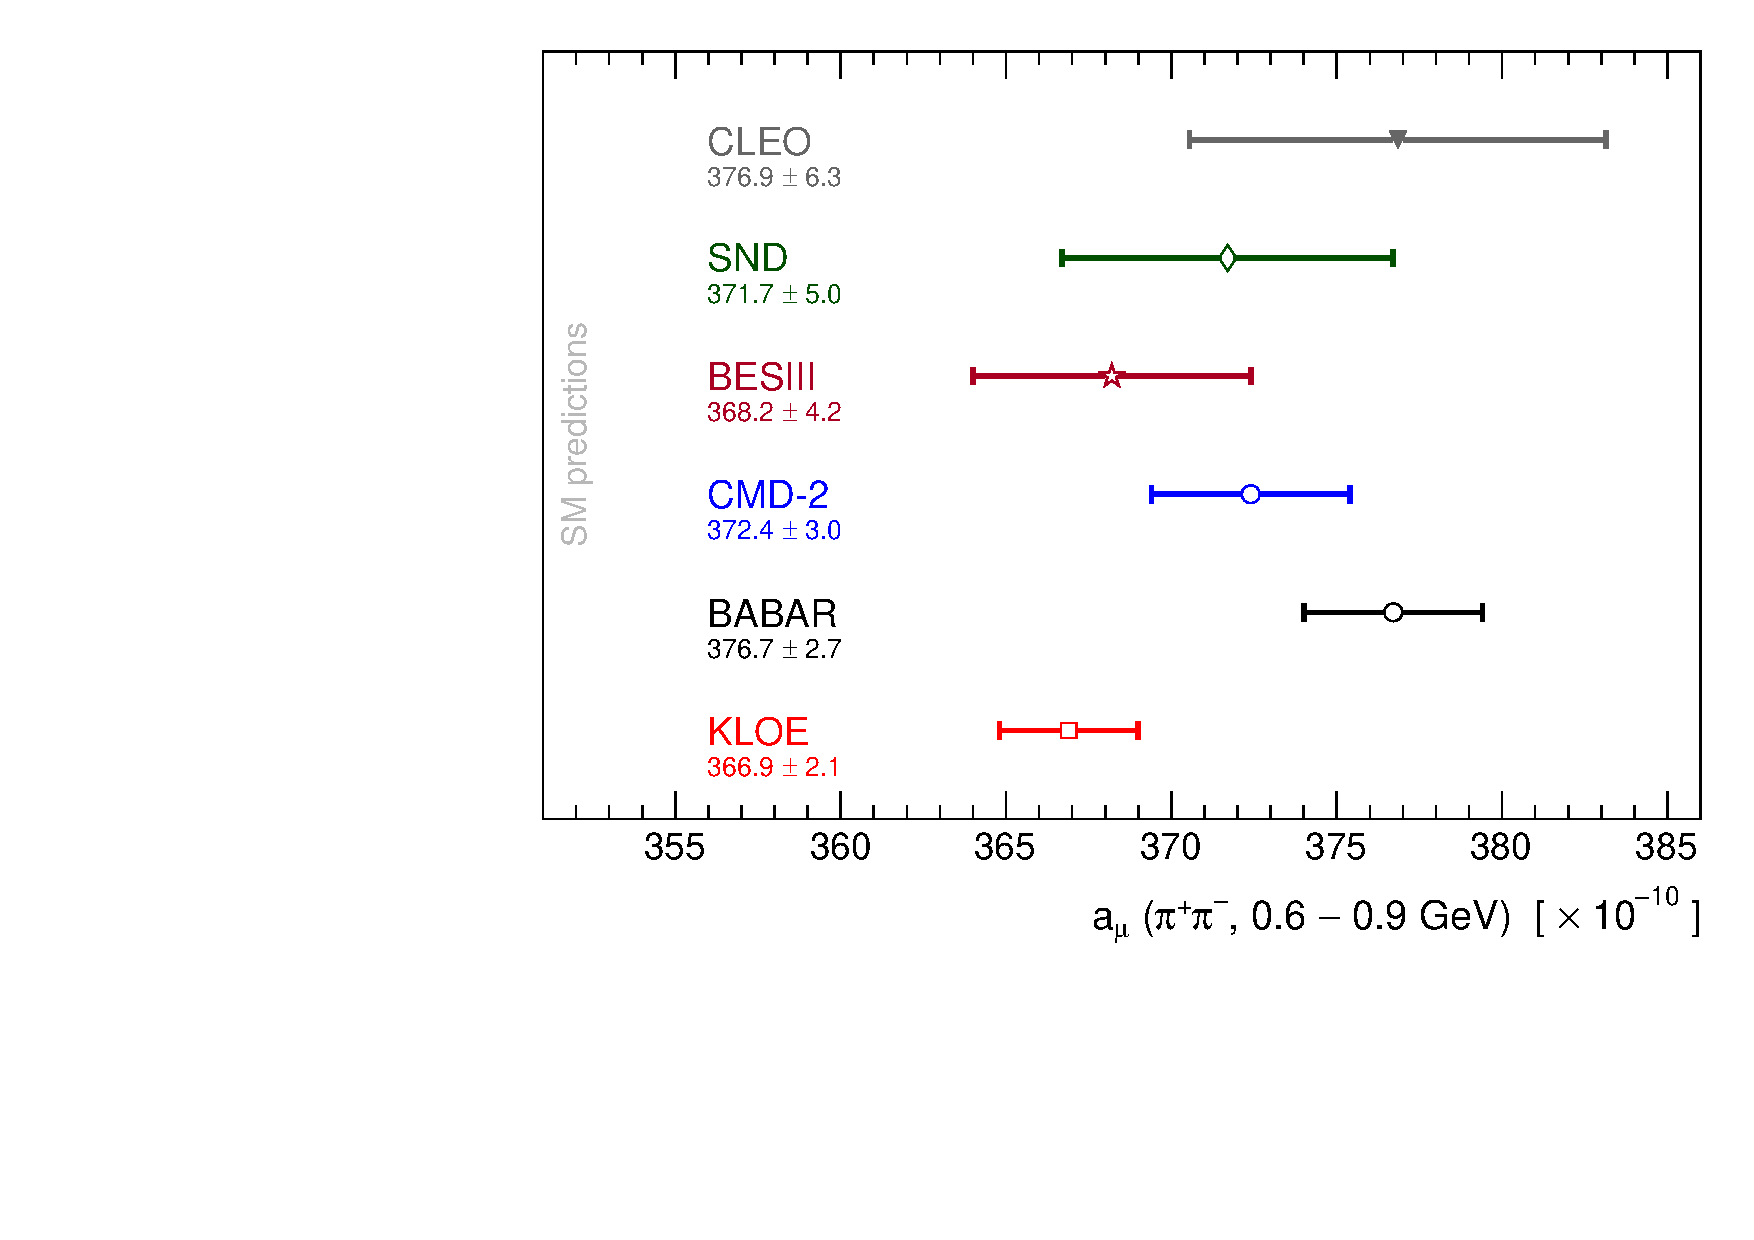
\includegraphics[width=\figsize]{Figures/amu2pi.pdf}
\end{center}
  \vspace{-0.15cm}
  \caption{Comparison of results for \amuhadLOpp, evaluated between 0.6$\;$GeV and 0.9$\;$GeV for the various experiments. In case of CMD-2 all available measurements have been combined using HVPTools. For KLOE the result from the public combination~\cite{kloe17} is displayed.}
  \label{fig:amu2pi}
\end{figure}
\begin{figure}[t]
\vspace{0.4cm}
\begin{center}
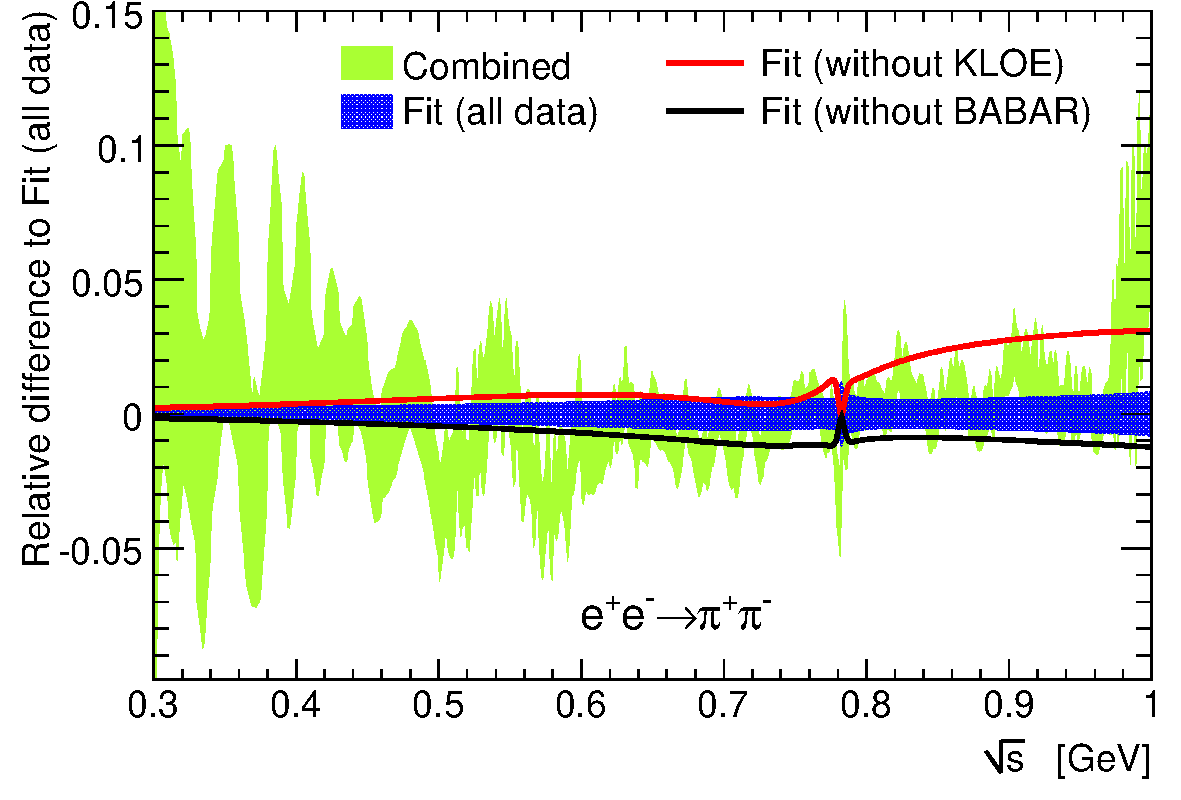
\includegraphics[width=\figsize]{Figures/ff2_comp_dhmz19.pdf}
\end{center}
  \vspace{-0.3cm}
  \caption{The HVPTools combination (green band) relative to the result of the fit to all individual $\pp$ data (blue band)  versus centre-of-mass energy. The black and red curves show the results of two alternative fits where the data from KLOE and BABAR, respectively,   were excluded.}
  \label{fig:ff2_comp}
\end{figure}
The evaluation of the complete \amuhadLOpp integral for the \pp contribution from threshold to 1.8$\;$GeV, using the fit up to 0.6$\;$GeV and the HVPTools data combination above, gives $507.0\pm1.9$. The choice of the ranges is justified by the good agreement between fit and combined data integration in the 0.6--1.0$\;$GeV region with, however, no advantage in precision for the fit. The correlation among the two contributions is found to be 62\% using pseudo-experiments.

Removing BABAR or KLOE from the dataset gives $505.1\pm2.1$ and $510.6\pm2.2$, respectively, with an absolute difference of 5.5 that is significantly larger than the individual uncertainties. Figure~\ref{fig:amu2pi} shows a comparison among the most precise \amuhadLOpp evaluations in the interval 0.6--0.9$\;$GeV. The results of all other experiments fall in-between the BABAR and KLOE results, with insufficient precision to resolve the discrepancy. 

Figure~\ref{fig:ff2_comp} compares the HVPTools combination and the fits without using the BABAR  and KLOE data, respectively, with the fit result for the full dataset. In light of this discrepancy, which is not fully captured by the local uncertainty rescaling procedure, we add as additional systematic uncertainty half of the full difference between the complete integrals without BABAR and KLOE, respectively, and we place the central value of the \amuhadLOpp contribution half-way between the two results. To avoid double counting, the local uncertainty rescaling between BABAR and KLOE is not applied, but that between these and the other \pp datasets is kept.
This procedure results in a total \pp contribution of  $\amuhadLOpp=507.9\pm0.8\pm3.2$, where the first uncertainty is statistical and the second systematic (dominated by the new uncertainty of 2.8).

\subsection{The \sansmath$\mathbf{\boldsymbol{K^+K^-}}$ channel}

Tensions among datasets are also present in the $K^+K^-$ channel (see top panel of Fig.~\ref{fig:kkweights} for a display of the available measurements). A discrepancy between BABAR and SND was observed for masses between 1.05 and 1.4$\;$GeV, which has been resolved with the most recent SND result~\cite{snd-kpkm} so that older SND data are discarded. 

Concerns also arise regarding data on the $\phi$(1020) resonance. Previously, a 5.1\% difference between CMD-2 at VEPP-2M and BABAR was observed, with the CMD-2 data being lower. New results from CMD-3 at VEPP-2000~\cite{Kozyrev:2017agm} exhibit the opposite effect: they are 5.5\% higher than BABAR (cf. middle panel in Fig.~\ref{fig:kkweights}). The  discrepancy of almost 11\% between the  CMD-2 and CMD-3 datasets, which largely exceeds the  quoted systematic uncertainty of 2.2\%, of which only 1.2\% accounts for uncertainties in the detection efficiency, is claimed to originate from a better understanding of the detection efficiency of low-energy kaons in the CMD-3 data.\footnote{In comparison with the CMD-2/3 and SND measurements, the ISR method of BABAR benefits from higher-momentum kaons with better detection efficiency owing to the boost of the final state.}
Given the  yet unresolved situation, we keep both CMD-2 and CMD-3 datasets, which due to the uncertainty rescaling procedure in presence of discrepancies leads to a deterioration of the precision by about a factor of two of the combined data (cf. bottom panel of Fig.~\ref{fig:kkweights}).\footnote{We have verified that the local $\chi^2$ rescaling procedure covers the global discrepancy among the CMD-2 and CMD-3 data by removing alternatively one or the other dataset from the $\Kp\Km$ combination. The difference of 0.45 resulting between the two $a_\mu$ values is covered by the uncertainty rescaling (a similar conclusion is reached for \dahadZ). There is therefore no need to introduce an additional global systematic uncertainty as for the $\pp$ case.}
% Due to the fact that the discrepancy occurs in the narrow phi mass region we expect the standard local chi2 scaling factor to cover well the effect. In addition the largest weight is from BABAR which helps stabilizing the result. 
\begin{figure}[p]
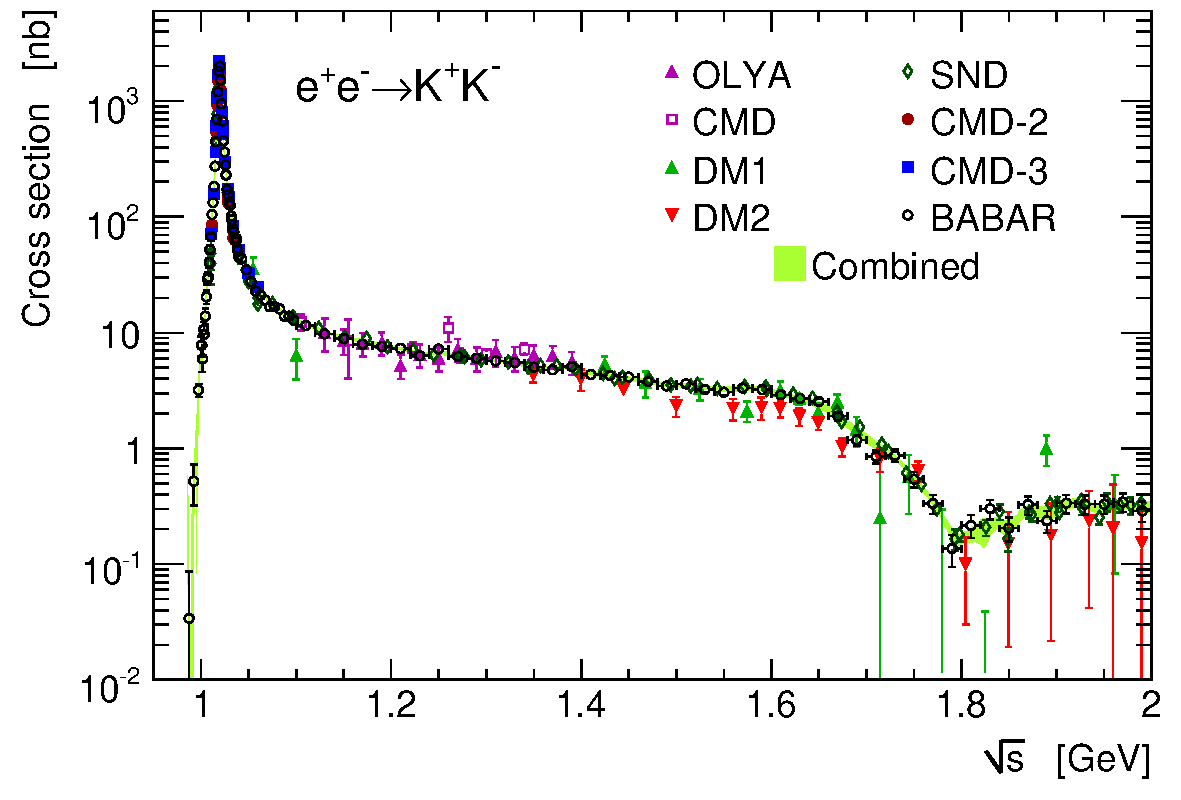
\includegraphics[width=\figsize]{Figures/combined_2pi_ePeM_to_phi_X__to_KPKM_X_log0,9-2,5GeV_dhmz19.pdf}
  \vspace{0.1cm}

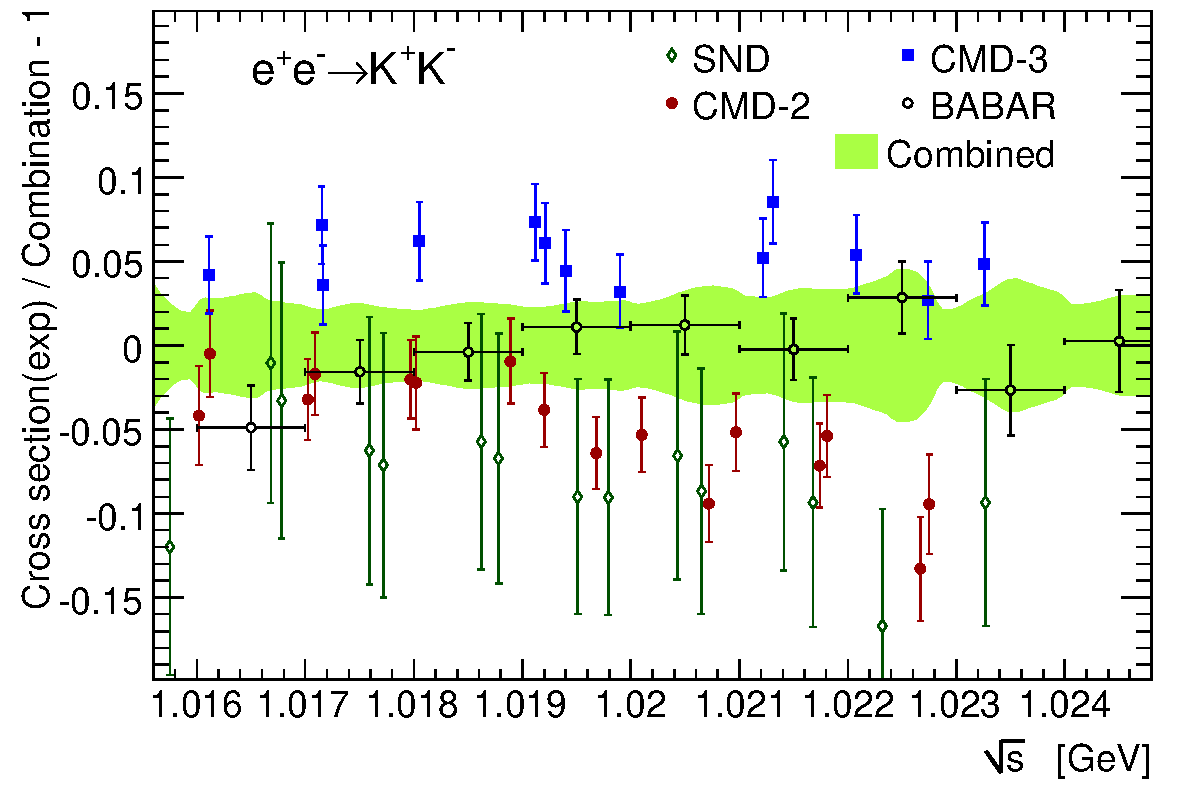
\includegraphics[width=\figsize]{Figures/diffRel_channel_ePeM_to_phi_X__to_KPKM_X_dhmz19.pdf}\hspace{\fighspace}

  \vspace{0.1cm}
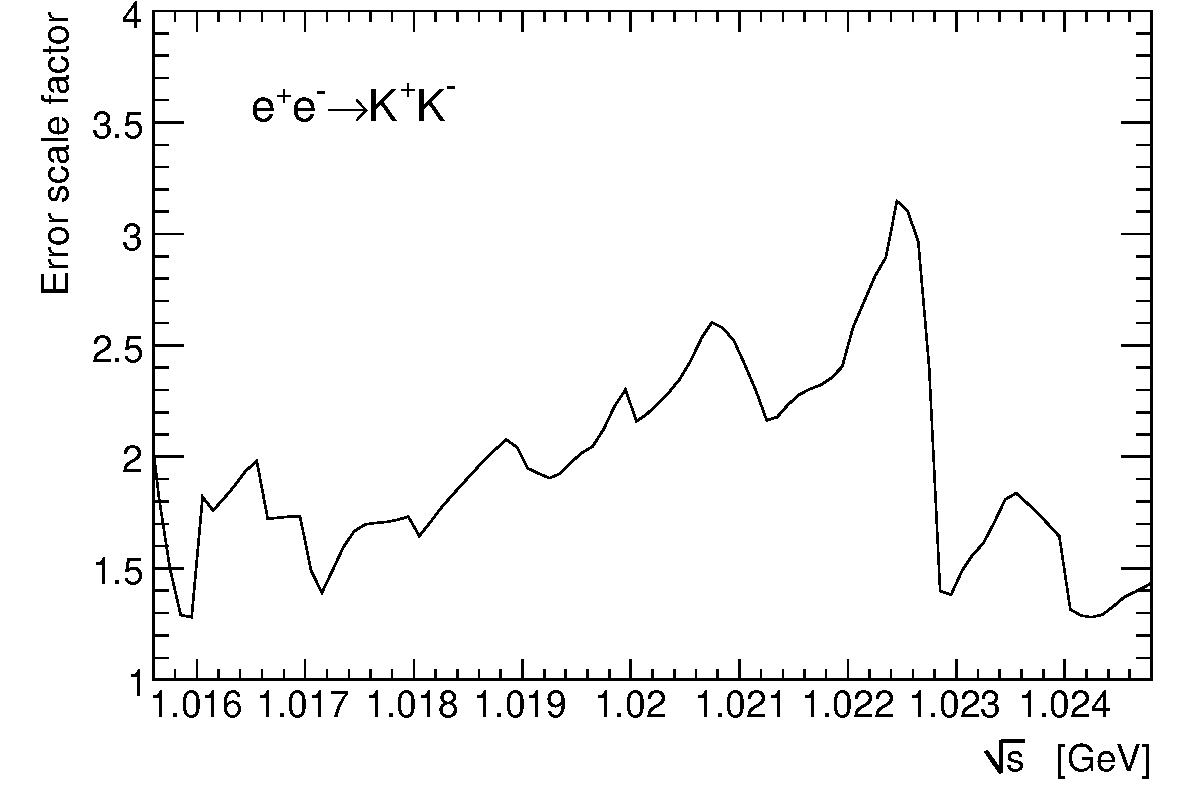
\includegraphics[width=\figsize]{Figures/Chi2Correction_combined_ePeM_to_phi_X__to_KPKM_X_dhmz19.pdf}
\vspace{-0.1cm}

\caption[.]{ 
            Top panel: bare cross sections for  $e^+e^-\to K^+ K^-  $. See text for a description of the data used. 
            Middle: comparison between individual $\ee\to K^+K^-$ cross-section measurements from BABAR~\cite{babar-kpkm}, CMD-2~\cite{Akhmetshin:2008gz}, CMD-3~\cite{Kozyrev:2017agm} and SND~\cite{snd-kpkm}, and the HVPTools combination.  
            Bottom: local scale factor versus centre-of-mass energy applied 
            to the combined $K^+K^-$ cross-section uncertainty to account for inconsistency 
            in the individual measurements. }
\label{fig:kkweights}
\end{figure}


\subsection{Other channels}

Recent measurements have been included in the data combinations: $\pi^0 \gamma$ from SND~\cite{Achasov:2018ujw}, $\pi^+\pi^-2\pi^0$ from BABAR~\cite{TheBaBar:2017vzo},  $\pi^+\pi^-3\pi^0$ from BABAR~\cite{Lees:2018dnv}, $\eta\pi^+\pi^-$ from BABAR~\cite{TheBABAR:2018vvb}, $\eta\pi^+\pi^-\pi^0$ from CMD-3~\cite{CMD-3:2017tgb} and SND~\cite{Achasov:2019duv}, $\phi\eta$ from CMD-3~\cite{Ivanov:2019crp}, and $K_SK_L\pi^0$ from SND~\cite{Achasov:2017vaq}.
The  $\pi^0 \gamma$ and $\pi^+\pi^-\pi^0$ contributions include small additions of $0.12\pm 0.01$ and $0.01\pm 0.00$, respectively, to cover the threshold region up to the lowest-energy data measurements~\cite{hmnt03,knt19}.

Only very few final states remain to be estimated using isospin symmetry. Already in 2017, a significant step was achieved with the BABAR measurements of all the final states contributing to the $K \Kbar \pi$ and $K \Kbar \pi\pi$ channels, so that previous isospin-based estimates became obsolete. Now the only significant (albeit small) contribution obtained with the use of isospin constraints is that for the $\pi^+\pi^-4\pi^0$ channel. The part excluding $\eta 3\pi$, which is obtained from measured processes and reevaluated in this analysis, amounts to a fraction of the total dispersion integral of only 0.016\% with an assigned systematic uncertainty of 100\%. One could also question the completeness of the set of exclusive processes considered below 1.8 GeV, including up to 6-pion and 
$K \Kbar$+3 pions. A recent measurement of the $3\pi^+ 3\pi^- \pi^0$ cross section by CMD-3~\cite{cmd3-7pi} allows one to estimate a very small total 7-pion contribution, included in this analysis, of only 0.002\%. Although such high-multiplicity channels appear to be contributing negligibly below 1.8$\;$GeV their importance is likely to increase above.

All other contributions are identical to the ones described in our previous analysis~\cite{dhmz2017}, except for (i) a reevaluation of the contribution from $\omega$ decay modes not reconstructed in other exclusive channels, and (ii) a better estimate of the $K \overline{K} \pi^+ \pi^- \pi^0$ contribution, excluding $\phi\eta$ which is dominated by the $K \overline{K} \omega$ final state~\cite{Aubert:2007ef}.
